\section{Introduction}

\subsection{Docker setup}
\nblink{brats3D/01\_preprocess.ipynb}
correctly symblink files, execute container, copy out result file

\subsection{Zero out cubes}
\nblink{brats3D/02\_generate\_slices.ipynb}
iterate over everything, zero cubes

\begin{figure}[H]
\centering
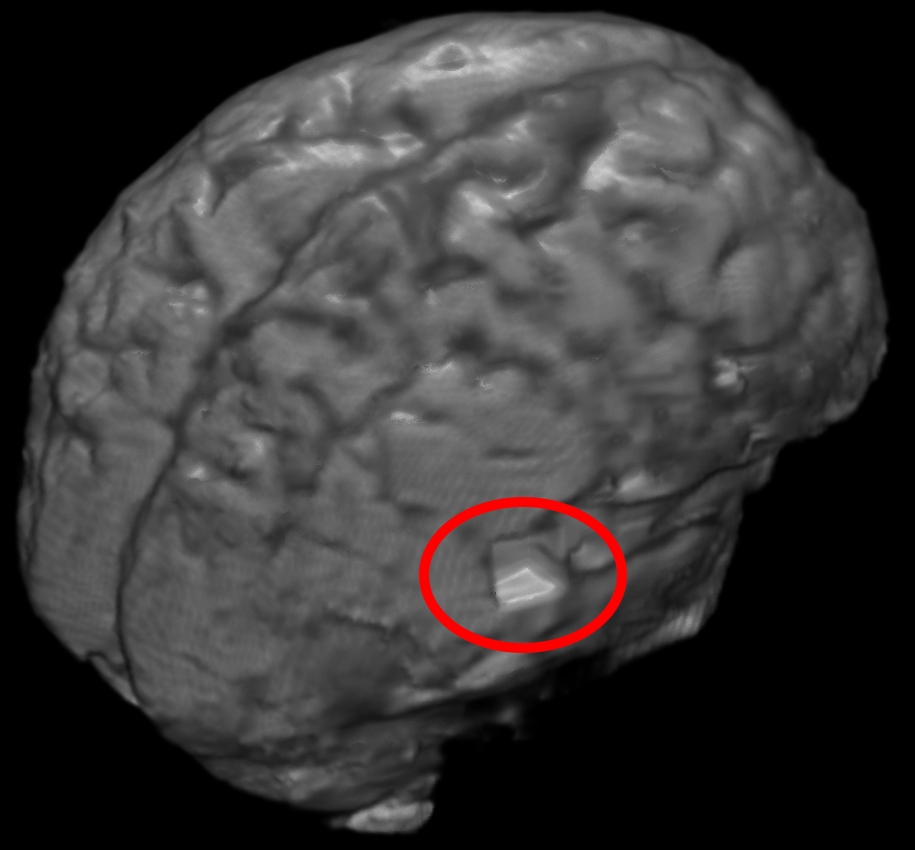
\includegraphics[width=10cm]{chapters/07_brats3d/images/brain-hdm-marked.png}
\caption{Modified scan with removed cube (red circle)}
\end{figure}


\subsection{Docker execution}
\nblink{brats3D/03\_execute.ipynb}
link up files

\subsection{Distance calculation}
\nblink{brats3D/04\_calculate\_hausdorff\_distance.ipynb}
hausdorff + MSE

\subsection{Visualization}
We use cubes, do not bother with circles just upscale pixels

\subsection{Results}
\nblink{brats3D/02a\_generate\_single\_slice.ipynb}
\nblink{brats3D/06\_display\_single\_slice.ipynb}

\begin{figure}[H]
    \centering
    \begin{subfigure}{.33\textwidth}
        \centering
        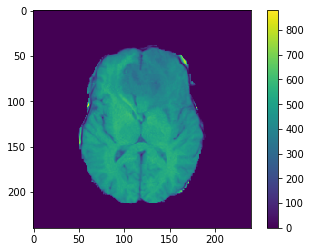
\includegraphics[width=\linewidth]{chapters/07_brats3d/images/01_t1.png}
        \caption{T1 modality of the slice}
    \end{subfigure}%
    \begin{subfigure}{.33\textwidth}
        \centering
        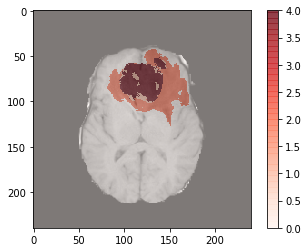
\includegraphics[width=\linewidth]{chapters/07_brats3d/images/05_t1_segment.png}
        \caption{T1 modality overlaid with ground truth tumor segment}
    \end{subfigure}
        \begin{subfigure}{.33\textwidth}
        \centering
        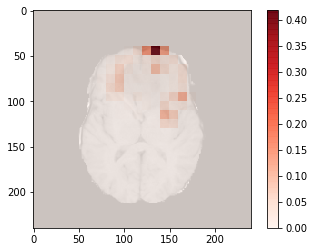
\includegraphics[width=\linewidth]{chapters/07_brats3d/images/09_t1_hdm10.png}
        \caption{T1 modality overlaid with hausdorff distance mask output}
    \end{subfigure}
    \caption{Visualization of the hausdorff distance mask result of the T1 modality. No big correlation between hausdorff distance mask output and actual tumor.}
\end{figure}

\begin{figure}[H]
    \centering
    \begin{subfigure}{.33\textwidth}
        \centering
        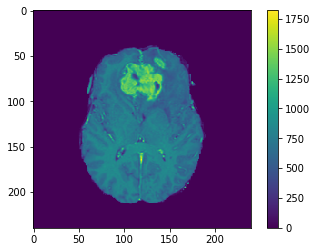
\includegraphics[width=\linewidth]{chapters/07_brats3d/images/02_t1ce.png}
        \caption{T1 contrast enhanced modality}
    \end{subfigure}%
    \begin{subfigure}{.33\textwidth}
        \centering
        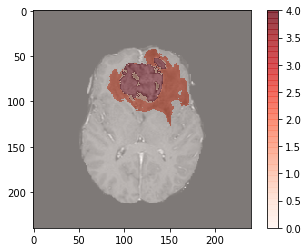
\includegraphics[width=\linewidth]{chapters/07_brats3d/images/06_t1ce_segment.png}
        \caption{T1 ce modality overlaid with ground truth tumor segment}
    \end{subfigure}
        \begin{subfigure}{.33\textwidth}
        \centering
        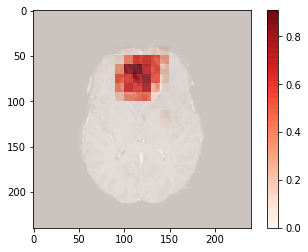
\includegraphics[width=\linewidth]{chapters/07_brats3d/images/10_t1ce_hdm.png}
        \caption{T1 ce modality overlaid with hausdorff distance mask output}
    \end{subfigure}
    \caption{Visualization of the hausdorff distance mask result of the T1 constract enhacned modality}
\end{figure}


\begin{figure}[H]
    \centering
    \begin{subfigure}{.33\textwidth}
        \centering
        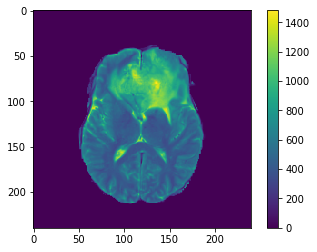
\includegraphics[width=\linewidth]{chapters/07_brats3d/images/03_t2.png}
        \caption{ the text for a}
    \end{subfigure}%
    \begin{subfigure}{.33\textwidth}
        \centering
        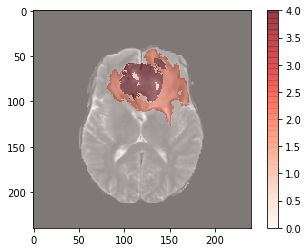
\includegraphics[width=\linewidth]{chapters/07_brats3d/images/07_t2_segment.png}
        \caption{b}
    \end{subfigure}
        \begin{subfigure}{.33\textwidth}
        \centering
        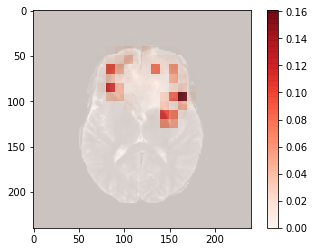
\includegraphics[width=\linewidth]{chapters/07_brats3d/images/11_t2_hdm.png}
        \caption{b}
    \end{subfigure}
    \caption{T2}
\end{figure}

\begin{figure}[H]
    \centering
    \begin{subfigure}{.33\textwidth}
        \centering
        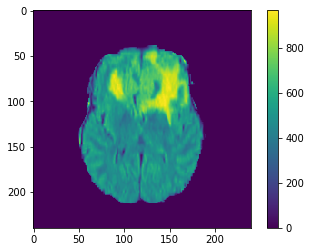
\includegraphics[width=\linewidth]{chapters/07_brats3d/images/04_flair.png}
        \caption{ the text for a}
    \end{subfigure}%
    \begin{subfigure}{.33\textwidth}
        \centering
        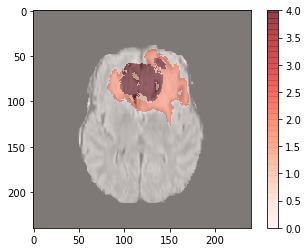
\includegraphics[width=\linewidth]{chapters/07_brats3d/images/08_flair_segment.png}
        \caption{b}
    \end{subfigure}
        \begin{subfigure}{.33\textwidth}
        \centering
        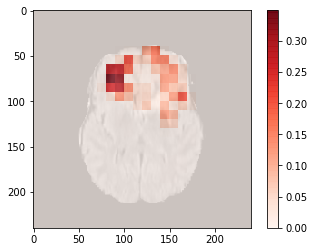
\includegraphics[width=\linewidth]{chapters/07_brats3d/images/12_flair_hdm.png}
        \caption{b}
    \end{subfigure}
    \caption{Flair}
\end{figure}

\subsection{Discussion}


\subsection{Conclusion}
